%======================================================================
\chapter{Details about the Method}
\label{chap:dm}
%======================================================================

In this chapter, we explain the details about our proposed method.
First of all, we give an overview of the framework, and identify the parts that compose the framework. Moreover, some parts have already been studied in our previous work, while some parts need to be explored in the future.
Second, we discuss the communication schema design of our framework.
Third, we demonstrate the pose estimation of multiple objects, which will be used in our framework.
Last, the limitations of the proposed framework are discussed.

\section{Overview}
\label{sec:dm:ov}

Figure~\ref{fig:ar-training-overview} shows the overview of the proposed AR training framework. It consists of five parts: 1) video capture; 2) video object segmentation; 3) pose estimation; 4) remote rendering; 5) synchronization.
The five parts form a loop that is repeated during the training process.

On the trainer side, the environment is captured as a monocular RGB video. In every loop, a captured frame is sent to the server.
The server is responsible for segmenting the moving objects from the frame. In the segmentation process, the information calculated from previous frames is considered to ensure temporal consistency of the segmentation.
In the pose estimation part, poses of all the moving objects in the current frame are calculated.
With the pose information, the framework is able to render all the moving objects for each trainee, with respect to their respective views.
In the synchronization part, a rendered frame that contains the virtual objects are sent to each client and overlapped on his/her real view.

\begin{figure*}[!htbp]
	\centering
	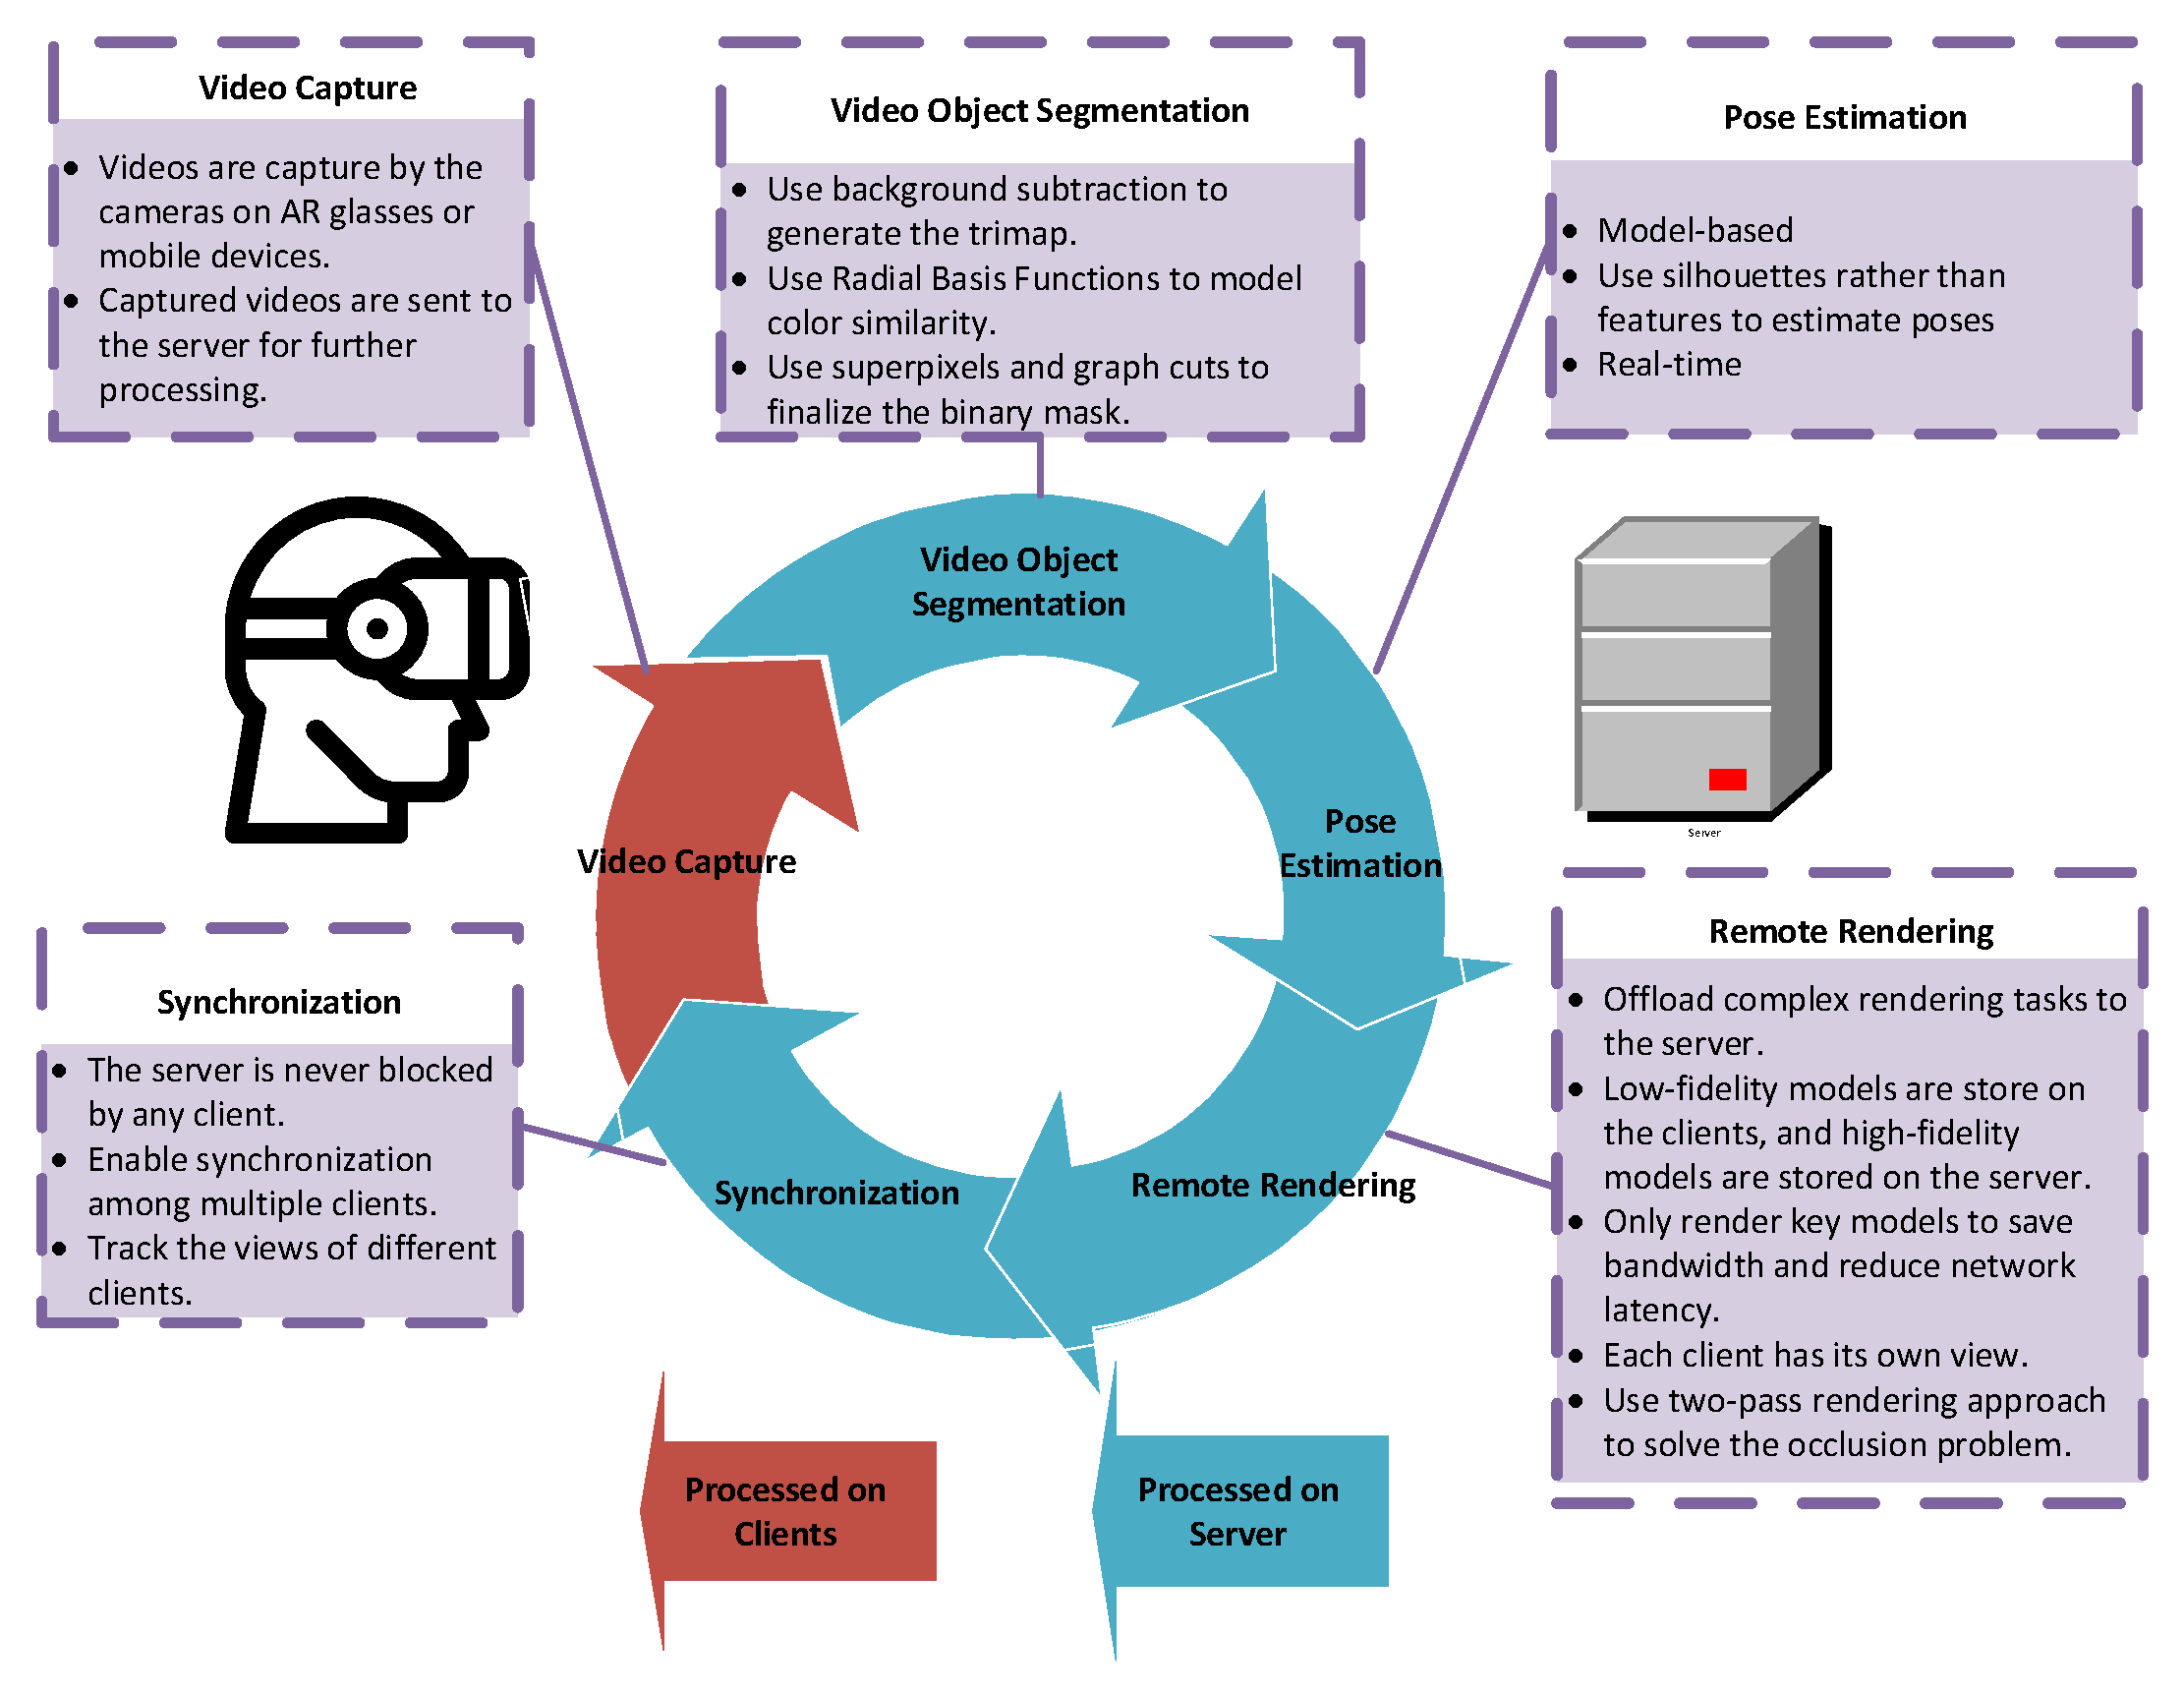
\includegraphics[width=\textwidth]{figures/AR-training-overview.pdf}
	\caption{Overview of the AR training framework. In the circle, the red arrow shows the part performed on the client side, i.e., AR glasses or mobile devices, while the blue arrows show the parts performed on the server side. In this way, the computing cost of the clients is minimized.}
	\label{fig:ar-training-overview}
\end{figure*}

On the trainee side, the procedure is similar.
The environment of every trainee is captured and sent to the server for segmentation and pose estimation.
Then, the moving objects from all the trainees are rendered on the server with respect to the trainer's view.
Last, a rendered frame that contains all the virtual objects are sent to the trainer's AR glasses or mobile devices and overlapped on his/her real view. During this step, virtual objects from different trainees can be marked by colors or markers.

Next, we discuss the details of each part.
% first
First of all, in the video capture part, the videos are captured by camera equipped AR glasses or mobile devices.
The cameras are monocular RGB cameras. In every loop, only one frame is captured.
Moreover, the captured frame is sent to the server for further processing.

% second
Second, for video object segmentation, we use background subtraction to generate a trimap that  roughly segments the frame into three regions: a) a definite foreground; b) a definite background; c) a blended region where pixels are considered as a mixture of foreground and background colors.
Then, we use Radial Basis Functions to model color similarity. After this step, every pixel is assigned a value that is the distance between the pixel and the foreground and the background based on a color similarity metric between every pixel in the blended region and the definite regions.
Furthermore, we clearly label each pixel as foreground or background using superpixles and graph cuts.

% third
Third, for pose estimation part, we use a model-based algorithm that uses silhouettes of objects to estimate poses~\cite{tjaden2016}.
It is a real-time algorithm.
However, the algorithm is estimating poses with known segmentations. In the original paper, it uses a level-set segmentation method and requires manual initialization of the segmentation.
In our framework, we use the video object segmentation method that we have created, which is also real-time.

% four
Four, AR glasses or mobile devices often have far less powerful graphics than desktop PCs or workstations.
To minimize the computing costs on the clients, we offload the complex rendering tasks to the server.
In the remote rendering method, low-fidelity models are stored on the clients, while high-fidelity models are stored on the server.
Because each client has its own view, the server must render a frame for each client.
To save bandwidth and reduce network latency, the server only renders key models. The rendered frames only contain the key model rendering results.
However, rendering only key models, we have to address the occlusion problem. We use a two-pass rendering approach to solve the problem.

% five
Last, in the synchronization part, we need a mechanism to manage communications between the clients and the server.
It must enable synchronization among multiple clients, and if a client fails to respond, the server must not be blocked.
Furthermore, it has the capacity to track the views of different clients

An advantage of our proposed framework is that, only video capture and relatively simple rendering are performed on the clients, while all the other parts are performed on the server.
In this way, the computing cost of the clients is minimized.

From Figure~\ref{fig:ar-training-overview}, we can see that, to realize the framework, there are three parts that need to be explored.
% first
The first is a video object segmentation part. In the work of Tjaden et al.~\cite{tjaden2016}, they use a level-set segmentation method and requires manual initialization of the segmentation.
Although there are existing automatic algorithms that are able to segment videos without manual initialization~\cite{brox2010,ochs2011,ochs2012,papazoglou2013,wang2015}, some methods are very slow~\cite{brox2010,ochs2011,ochs2012}, some are offline methods that require the availability of the entire video.
Thus, we propose a novel video object segmentation method that is real-time and offers online processing.
This part has been done, and the details about the method can be found in Chapter~\ref{chap:vos}.

% second
The second is a remote rendering method.
AR glasses and mobile devices usually have less graphics capacity, compared to desktop PCs and workstations.
We have proposed a remote rendering method that is compatible with multiple clients to minimize the computing costs of the clients. This work can be found in Chapter~\ref{chap:hrr}.

% third
Last, we need to design and implement a communication schema to manage communications between the clients and the server.
This schema must be able to synchronize the states of different clients and the server.
Moreover, it should have the capacity to track the views of different clients.
This part has not been implemented, and we draw the blueprint of the schema in Section~\ref{sec:dm:csd}.

\section{Communication Schema Design}
\label{sec:dm:csd}

As shown as Figure~\ref{fig-comm-schem}, the system consists of four services: control service, pose estimation service, rendering service and the encoding service.
The control service is responsible for controlling the entire process.
First of all, it sends requests to the pose estimation service to perform pose estimation for each client, including the trainer and all the trainees.
Note that the pose estimation service is a non-blocking service. It receives the video captured from each client independently and updates its estimation result right after receiving every frame from every client. In this way, it maintains a database of the relative pose of each object for each client. Every time it receives the request from the control service, it sends the current database to the control service.

Once the control service gets the result from the pose estimation service, it sends the pose estimation result and the rendering request to the rendering service.
When the rendering service finishes rendering the models of interest for all the clients according to their point of view, it sends back the rendering result to the control service.
Note that the models of interest include the models of the components whose state (i.e. position and orientation) has been changed by the trainer but not changed accordingly by the trainees. In other words, it means the components to which the trainer and the trainees need to pay attention.

Last, the control service sends the rendering result and encoding request to the encoding service. Once the encoding service has accomplished encoding, it sends the encoded frames to each client.
The encoding service is a non-blocking service. The control service does not need to wait for the response from it to continue the process.

\begin{figure*}[!htbp]
	\centering
	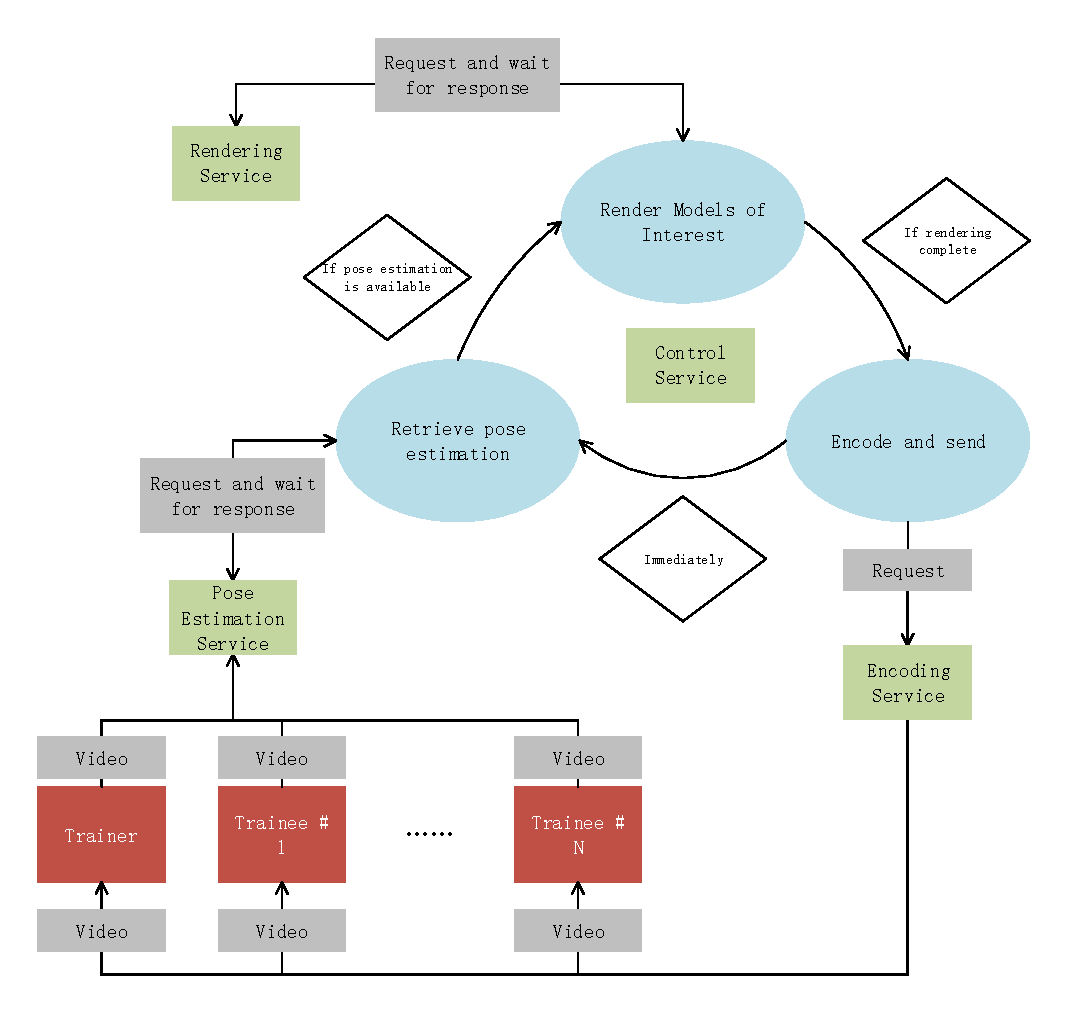
\includegraphics[width=\textwidth]{figures/communication_schema.pdf}
	\caption{Communication Schema}
	\label{fig-comm-schem}
\end{figure*}

As will be discussed in Chapter~\ref{chap:hrr}, our remote rendering method includes two types of models: high-fidelity models and low-fidelity models, where the high-fidelity models are stored on the server side while the low-fidelity models are stored on the client side. Thus, even without the rendering service, the clients are able to render the models if they have the basic rendering capacity.
In our schema, the only blocking service is the rendering service. For real-time performance, we set a time limit of $1/30$ second for the rendering service. If it does not accomplish the rendering within the time limit, the control service will send the pose estimation result to the clients and let them do the rendering themselves.

\section{Pose Estimation of Multiple Objects}
\label{sec:dm:pemo}

The first step towards our proposed framework is to estimate the poses of the objects of interest, namely the position and orientation of each object over time.
We use a model-based algorithm to estimate the poses.
With model-based pose estimation algorithms, the 3D structure of the objects of interest must be known beforehand. It is often the case in industrial training~\cite{cremers2007}.

% words need change
Some model-based approaches use edge or point features associated with the 3D models for estimating the pose~\cite{harris1990,vacchetti2004,park2008,kim2010}.
However, there are two major disadvantages with feature-based methods.
First, they struggle with motion blur and are prone to local minima, especially with cluttered backgrounds.
Second, using point-based features also requires the objects' surfaces to be sufficiently textured, which significantly limits the variety of suitable objects.

% words need change
Recently, region-based pose estimation methods have emerged, which are mainly based on statistical level-set segmentation approaches.
The main advantage is that they do not require sufficiently textured objects and only reply on structure of the objects.
However, this category of approaches only work in application scenarios where it is undesirable or even impossible to modify the objects. In other words, they require the objects to be rigid. It is often the case in industrial or manufacturing training.

% words need change
In~\cite{prisacariu2012}, the authors present PWP3D, the first region-based  approach that achieves real-time frame rates (20-25 Hz) using GPUs by solving the pose estimation similar to the variational approach suggested in~\cite{dambreville2010}, but using level-set functions instead of separately integrating over the foreground and background region to simplify computations and make it real-time capable.
Recently, another improved PWP3D version was proposed, which runs at 30 Hz on a mobile phone~\cite{prisacariu2015}.
Tjaden et al. built an algorithm based on PWP3D, which improves convergence properties, especially for rotational motion~\cite{tjaden2016}. Also, the described implementation that uses the GPU only for rendering purposes, and performs the rest computations on the CPU to achieve frame rates of about 50-100 Hz when tracking a single object on a commodity laptop.

Our method uses the work proposed by Tjaden et al.~\cite{tjaden2016} in our pose estimation service, where the object segmentation and pose estimation are performed in an interleaved fashion for each camera image.
However, the approach uses a level-set segmentation method and requires manual initialization of the segmentation, which limits its usage in real applications.
We proposed an automatic video object segmentation method, as described in Chapter~\ref{chap:vos}. In our work, the object segmentations are initialized automatically and it works with multiple objects.
Compared with other state-of-the-art automatic video object segmentation methods, our approach has the advantage that it runs in real-time.
Moreover, the synthetic silhouette that is generated with the models can be used as a ground truth segmentation, which will be used to improve the foreground and background segmentation results.

\section{Limitations}
\label{sec:dm:l}

However, the proposed framework still has several limitations.
First, the 3D models of objects involved in the training must be known beforehand, since the techniques we use in pose estimation are model-based.
The reason why we use a model-based pose estimation method is that this kind of methods are typically more accurate than those approaches that estimate the 3D structure and pose at the same time. Another advantage of using a model-based pose estimation method is that it does not require the presence of markers.
However, our proposed framework aims at training scenarios. In many cases the CAD models are typically known beforehand, such as in manufacturing and assembly tasks.
In some other training scenarios, an extra effort is needed to obtain the 3D structures of the objects involved.
Second, the proposed framework does not work with non-rigid bodies.
For instance, in surgery training, the organs are deformable, and thus, it is not enough to only track the translation and orientation of an organ.
